\documentclass{kuburgiearticle}

\usepackage{amsmath}
\usepackage{amssymb}
%\usepackage{amsfonts}
%\usepackage{amsthm}
%\usepackage{tcolorbox}
\usepackage{mathtools}
\usepackage{siunitx}
\usepackage{cancel}
%\usepackage{mathtools}
\usepackage[american, straightlabels, cuteinductors]{circuitikz}
\usepackage{subcaption}

%\DeclareUnicodeCharacter{}{I~AM~HERE!!!!}

\let\epsilon\varepsilon

\newcommand{\R}{\mathbb{R}} % Real numbers
\newcommand{\C}{\mathbb{C}} % Complex numbers
\newcommand{\Q}{\mathbb{Q}}
\newcommand{\N}{\mathbb{N}}

\DeclarePairedDelimiter\abs{\lvert}{\rvert}
\usepackage{array}
\usepackage{multirow}

\sisetup{output-decimal-marker={.}}
\sisetup{per-mode=power}
\sisetup{group-digits=integer}

\newcommand{\rood[1]}{\color{red}#1\color{black}}

\usepackage[dutch]{babel}
\usepackage{hyperref}

%\setlength{\parindent}{0pt}
% d voor dx
\newcommand*\diff{\mathop{}\!\mathrm{d}}

\usepackage{parskip}

\title{Examen Elektrische Netwerken}
\author{Vincent Van Schependom}
\date{20 januari 2025}
\address{
	\textbf{Elektrische Netwerken}\\
	X0E58A\\
	Ben Hermans}

\begin{document}

	\maketitle

	\section*{Tips voor onze opvolgers}

	\begin{itemize}
		\item Lees goed het voorblad!
		\item Schrijf niet op de kladbladen, want die worden niet verbeterd. Je moet al je antwoorden op de opgavebundel schrijven (er is voldoende plaats voorzien).
		\item Werk door. Het examen is véél te uitgebreid om op 3 uur tijd helemaal af te werken. Ik raad aan om bij grote `bepaal de beschrijving' achtige oefeningen (zoals Oefening 1 van dit examen) alle vergelijkingen op te schrijven, maar ze nog niet meteen op te lossen. Laat dit voor het einde. Als je op miraculeuze wijze nog tijd zou over hebben, kan je ze eventueel verder uitwerken.
	\end{itemize}

	\newpage

	\section*{Vraag 1}

	\begin{figure}[h!]
		\centering
		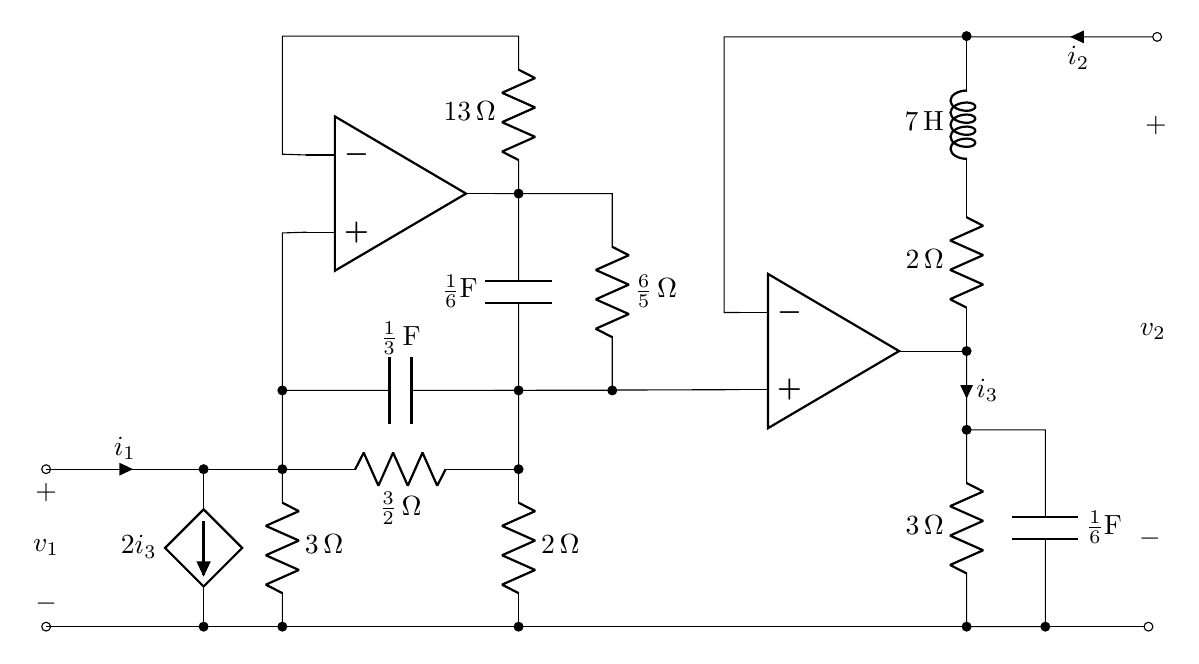
\begin{tikzpicture}
		\draw (10,3.5) node[op amp] (opamp) {};

		\draw (0,2) node[] (vtop) {} to[open, o-o, v=$v_1$] (0,0) node[] (vbottom) {};

		\draw (vtop.center) to[short, -*, i=$i_1$] ++ (2,0) node[] (i3) {}
							to[short, -*] ++ (1,0) node[] (weerstand1) {}
							to[short, -*, R, l_=$\frac{3}{2}\,\unit{\ohm}$] ++ (3,0) node[] (weerstand2) {};

		\draw (i3.center) to[short, -*, controlled isource, l_=$2i_3$] ++ (0,-2);
		\draw (weerstand1.center) to[short, -*, R, l=$3\,\unit{\ohm}$] ++ (0,-2);
		\draw (weerstand2.center) to[short, -*, R, l=$2\,\unit{\ohm}$] ++ (0,-2);

		\draw (opamp.-) to[short] ++ (-0.2,0)
						to[short] ++ (0,3.5)
						to[short, -] ++ (3.5,0)
						to[short, -o, i<_=$i_2$] ++ (2,0) node [] (v2top) {};

		\draw (weerstand1.center) to[short, -*] ++ (0,1) node [] (condensator1) {}
								  to[short, -*, C, l=$\frac{1}{3}\,\unit{\farad}$] ++ (3,0) node [] (z) {}
								  to[short] ++ (0,-1);

		\draw (condensator1) ++ (1.5, 2.5) node[op amp] (opamp2) {};

		\draw (z.center) to[short, -*, C, l=$\frac{1}{6}\unit{\farad}$] ++ (0, 2.5) node [] (out) {}
						to[short] (opamp2.out)
						to[short, -] ++ (1.5,0)
						to[short, -*, R, l=$\frac{6}{5}\,\unit{\ohm}$] ++ (0,-2.5)
						to[short] ++ (-1.5,0)
						to[short] (opamp.+);

		\draw (out.center) to[short, R, l=$\SI{13}{\ohm}$] ++ (0,2)
						to[short] ++ (-3,0)
						to[short] ++ (0,-1.5)
						to[short] (opamp2.-);

		\draw (condensator1.center) to[short] ++ (0,2) to (opamp2.+);

		\draw (opamp.out) to[short,-*] ++ (0.5,0) node [] (zrechts) {}
							to[short, -] ++ (0,0.25)
							to[short, -, R, l=$2\,\SI{}{\ohm}$] ++ (0,1.75)
							to[short, L, l=$7\,\SI{}{\henry}$] ++ (0,1.75)
							to[short, -*] ++ (0,0.25);

		\draw (zrechts.center) to[short, -*, i=$i_3$] ++ (0,-1)
								to[R, l_=$3\,\unit{\ohm}$, -*] ++ (0,-2.5)
								to[short, -*] ++ (1,0)
								to[C, l_=$\frac{1}{6}\unit{\farad}$, -] ++ (0,2.5)
								to[short, -] ++ (-1,0);

		\draw (vbottom.center) to[short, -o] ++ (14,0) node[] (v2bottom) {};
		\draw (v2top) to[open, v=$v_2$] (v2bottom);

	\end{tikzpicture}
	\end{figure}

	\vspace{0.5cm}

	\begin{enumerate}
		\item[a)] Bepaal een beschrijving van bovenstaande tweepoort.
		\item[b)] Welke beschrijvingen bestaan nog? Antwoord in één zin.
		\item[c)] Bepaal het Thévenin-equivalent indien we de tweepoort afsluiten met een spanningsbron van \({i_2=\SI{2}{\ampere}}\). Als deze niet bestaat, geef dat dan duidelijk aan.
	\end{enumerate}

	\vspace{2cm}

	\subsection*{Tips voor onze opvolgers:}
	\begin{itemize}
		\item Er staat al een behoorlijk deel van de punten op het correct neerschrijven van alle vergelijkingen:
		\begin{itemize}
			\item De stroom- en spanningswetten
			\item De vergelijkingen van de opamps (\(i_- = i_+ = 0\), $e_-=e_+$ en $i_\text{out} = $ niet gekend).
		\end{itemize}
		Schrijf deze dus zeker \textit{allemaal} op -- ook degene die je eigenijk niet nodig hebt.
		\item Wanneer je de beschrijving zoekt, is het onbegonnen werk om gewoon wat random vergelijkingen te beginnen substitueren in andere vergelijkingen. Kijk goed naar wat je nodig hebt:
		\begin{itemize}
			\item Je wil een uitdrukking met \(i_1, i_2, v_1\) en \(v_2\). Je kan -- door het netwerk kritisch te analyseren -- de spannings- / stroomdeler toepassen; zo vind je vrij snel een beschrijving.
		\end{itemize}
		\item Als je de beschrijving niet zou gevonden hebben, vermeld dan zeker hoe je vraag b) zou oplossen: je kijkt waar er al dan niet gedeeld wordt door nul. Als er zo'n deling door nul optreedt, bestaat de beschrijving in kwestie niet. Alleen dit levert al een half punt op!
		\item Dit volgt de lijn van het vorig puntje: als je het equivalent niet gevonden hebt, schrijf dan gewoon op hoe een Thévenin equivalent er precies uitziet (let op met DC/AC!) en leg uit hoe je dit zou bepalen (alle onafhankelijke bronnen op nul, \(R_\text{eq}=v/i\), ...).
	\end{itemize}

	\newpage

	\section*{Vraag 2}

	\vspace{-0.5cm}
	\begin{figure}[h!]
		\centering
		\begin{subfigure}{.49\textwidth}
			\centering
				\begin{tikzpicture}
				\draw (0,0) to[short, *-, R, l=$R_1$] (0,2.5) node[](links){}
				to[short, *-] (0,3) node[](linksonder){}
				to[short, *-, I, l=$I_S$] ++ (3,0) node[](is){}
				to[short, *-] ++ (3,0);
				\draw (linksonder.center) 	to [*-, R, l=$R_2$] ++ (0,3) node[](linksboven){}
				to [*-, C, l=$C$] (is.center)
				to [*-, R, l=$R$] ++ (0,3);
				\draw (linksboven.center) to [short, *-, L, l=$L$] ++ (3,0)
				to [short, *-] ++ (3,0) node[](rechtsboven){}
				to [short, *-*, controlled current source, invert, l=$\alpha i_{R_1}$] ++ (0, -3) node[](rechtsonder){} to[short, -*] ++ (0,-0.5) node[](rechts){};
				\draw (3,6) to [short, *-, controlled isource, invert, l=$\beta v_{R_2}$, label position=above] ++ (3,-3);

				\node[draw, circle, minimum size=1cm] (raarelement) at (3,1) {};
				\draw (links.center) to[short] (raarelement.145) to[short] (raarelement.center);
				\draw (rechts.center) to[short] (raarelement.35) to[short] (raarelement.center);
				\draw (raarelement.center) to[short, -*] ++(0,-1) node[](middenonder){};

				\draw (0,0) to[short] (middenonder.center)
								to[short, *-*] ++ (3,0)
								to[short, -] ++ (0,0.25)
								to[short, -, vsource, invert, v_=$v_4$] ++ (0,1)
								to[short, -, vsource, invert, v_=$v_3$] ++ (0,1)
								to[short, -*] ++ (0,0.25);

			\end{tikzpicture}
			\caption{}
			\label{fig:a}
		\end{subfigure}
		\hfill
		\begin{subfigure}{.49\textwidth}
			\centering
			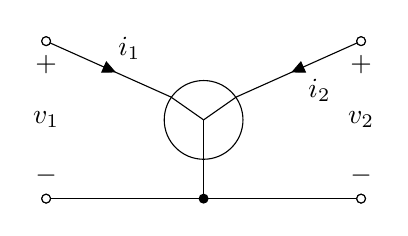
\begin{tikzpicture}

				\node[draw, circle, minimum size=1cm] (raarelement) at (2,1) {};

				\draw (0,2) node[](linksboven){} to[short, o-, i=$i_1$] (raarelement.145) to[short] (raarelement.center);
				\draw (4,2) node[](rechtsboven){} to[short, o-, i=$i_2$] (raarelement.35) to[short] (raarelement.center);
				\draw (raarelement.center) to[short, -*] ++(0,-1) node[](middenonder){};

				\draw (0,0) node[](linksonder){} to[short, o-] (middenonder.center)
				to[short, -o] ++ (2,0) node[](rechtsonder){};

				\draw (linksboven) to[open, o-o, v=$v_1$] (linksonder);
				\draw (rechtsboven) to[open, o-o, v=$v_2$] (rechtsonder);

			\end{tikzpicture}
			\caption{}
			\label{fig:b}
		\end{subfigure}
	\end{figure}

	Voer Modified Node Analysis uit op het circuit in (a), waarbij de karakteristiek van de tweepoort in (b) gegeven wordt door: \begin{align*}
		\begin{cases}
			v_1 = 6i_1 + 2i_2\\
			v_2 = 4i_1 + 3i_2
		\end{cases}
	\end{align*}
	Geef duidelijk aan wat je (niet) met gewone knooppuntanalyse kan bepalen.

	\newpage

	\newpage

	\section*{Vraag 3}

	\vspace{-0.5cm}

	\begin{figure}[h!]
		\centering
		\begin{circuitikz}
	\draw   (0,0) node[transformer] (T) {};

	% Input and output nodes
	\draw (T.A1) node[anchor=east, ocirc] (i) {}
	(T.A2) node[anchor=east, ocirc] (j) {}
	(T.B1) node[anchor=west, ocirc] (m) {}
	(T.B2) node[anchor=west, ocirc] (k) {};

	% Labels near terminals
	\draw (i) ++ (-0.15,0) node[anchor=east, circle, draw] {$i$}
	(j) ++ (-0.15,0) node[anchor=east, circle, draw] {$j$}
	(m) ++ (0.15,0) node[anchor=west, circle, draw] {$m$}
	(k) ++ (0.15,0) node[anchor=west, circle, draw] {$k$}

	% Transformer ratio label
	(T.base) node[above] {$n:1$};
\end{circuitikz}
	\end{figure}

	Beschouw de ideale transformator hierboven.

	\begin{enumerate}
		\item[a)] Welke beschrijvingen bestaan?
		\item[b)] Kunnen we deze component beschrijven met behulp van gewone knooppuntanalyse?
		\item[c)] Leid de stempel van de ideale transformator af.
	\end{enumerate}

	\newpage

	\section*{Vraag 4}
	\vspace{-0.8cm}
	\begin{figure}[h!]
		\centering
		\begin{circuitikz}
			\draw (0,0) node[] (top) {} to[short, o-*, C, l_=$C$, i>_=$I$] ++ (-1.5,0) node[] (weerstand3) {}
						to[short, -*] ++ (-1,0) node[] (weerstand2) {}
						to[short, -*] ++ (-1.5,0) node[] (source) {}
						to[short, -] ++ (-0.5,0)
						to[short, R, l=$R_1$] ++ (-1.5,0)
						to[short, L, l=$L$] ++ (-1.5,0)
						to[short, -] ++ (-0.5,0)
						to[short, vsource, l=$E_0$] ++ (0,-3)
						to[short, -o] ++ (8,0) node[] (bottom) {};

			\draw (weerstand2.center) to[short, -*, R,l_=$R_2$] ++ (0,-3);
			\draw (weerstand3.center) to[short, -*, R,l=$R_3$] ++ (0,-3);
			\draw (source.center) to[short, -*, controlled isource,l_=$2I$] ++ (0,-3);

			\draw (top) to[open, v=$V$] (bottom);
		\end{circuitikz}
	\end{figure}

	Teken het fasorendiagram van bovenstaand netwerk, ervan uitgaande dat \(I\neq 0\). Verder geldt dat \({\omega=\SI{1}{\radian\per\second}}, R_1=\SI{0.5}{\ohm}, R_2=\SI{1}{\ohm},R_3=\SI{1}{\ohm}\) en \(C=\SI{1}{\farad}\). De complexe amplitudes van \(E_0\) en \(I\) zijn respectievelijk \SI{2}{\volt} en \(\sqrt{2}\,\SI{}{\ampere}\).

	\vspace{1cm}

	\begin{figure}[h!]
		\centering
		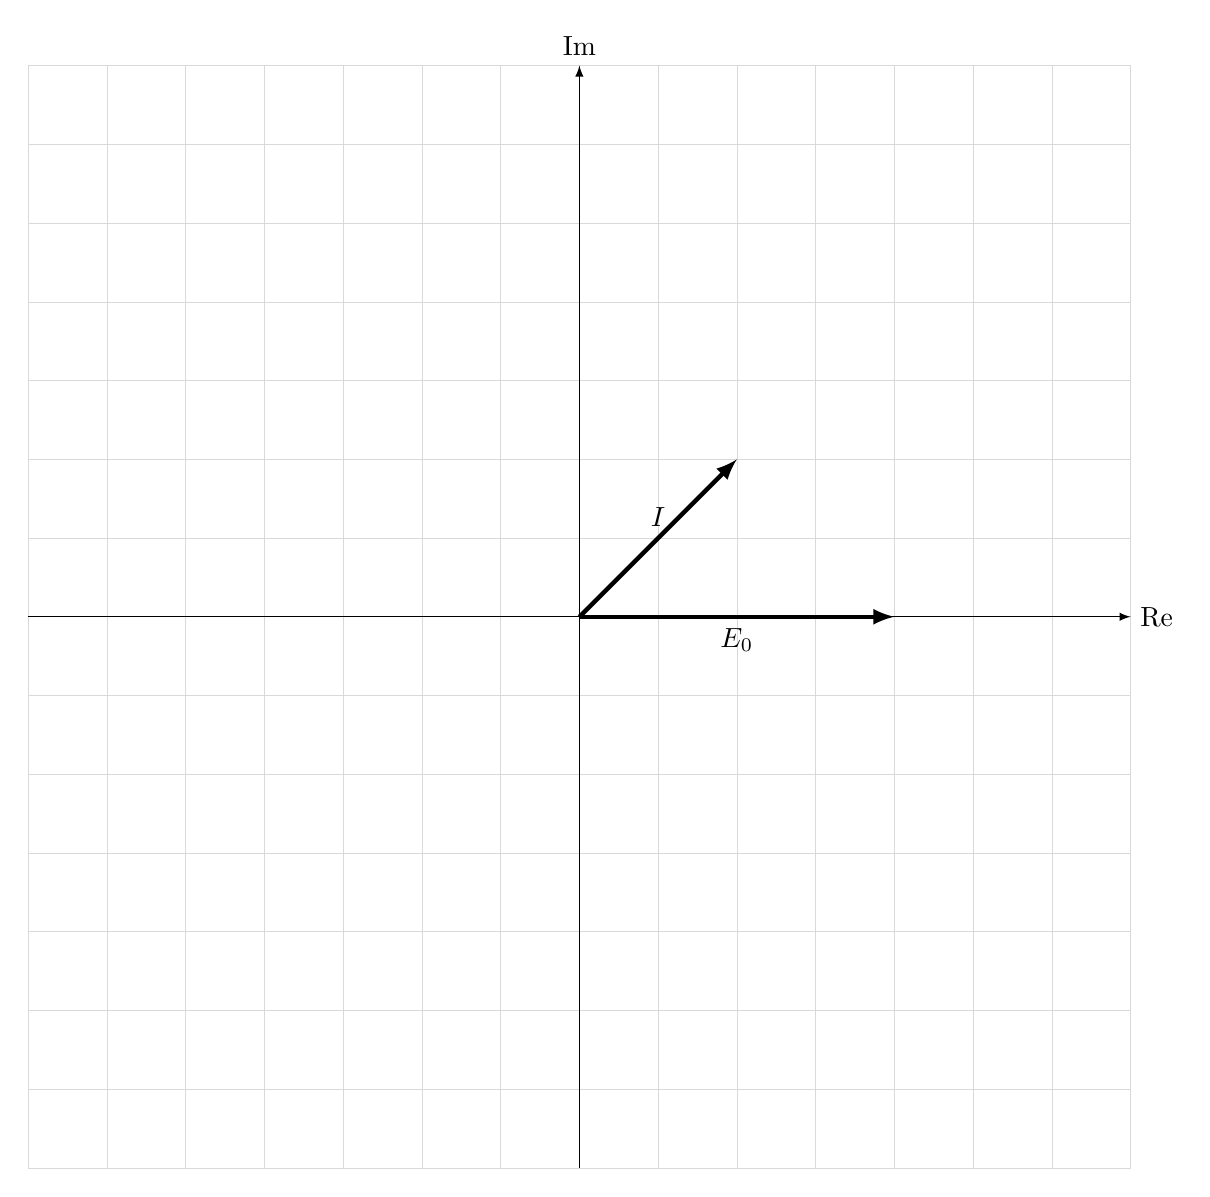
\begin{tikzpicture}
			\draw[help lines, color=gray!30] (-7,-7) grid (7,7);
			\draw[-latex] (-7,0)--(7,0) node[right]{Re};
			\draw[-latex] (0,-7)--(0,7) node[above]{Im};
			\draw[ultra thick, -latex] (0,0)--(2,2) node[midway,above] () {$I$};
			\draw[ultra thick, -latex] (0,0)--(4,0) node[midway,below] () {$E_0$};
		\end{tikzpicture}
	\end{figure}

	\newpage

	\section*{Vraag 5}

	\begin{figure}[h!]
		\centering
		\begin{subfigure}{.4\textwidth}
			\centering
			\begin{circuitikz}
				\draw (0,0) node[] (linksonder) {} to[short, o-] ++ (2,0)
				to[short, -*] ++ (0,1) node[] (onder) {};

				\draw (onder.center) 	to[short] ++ (-1,0)
				to[short] ++ (0,0.5)
				to[R, l=$\SI{1}{\ohm}$] ++ (0,1.5)
				to[diode, invert] ++ (0,1.5)
				to[short] ++ (0,0.5);

				\draw (onder.center) 	to[short] ++ (1,0)
				to[isource, l=$\SI{2}{\ampere}$] ++ (0,4)
				to[short, -*] ++ (-1, 0) node[] (boven) {}
				to[short] ++ (-1,0);

				\draw(boven.center) to[short, i=$i$] ++ (0,1)
				to[short, -o] ++ (-2,0) node[] (linksboven) {};

				\draw(linksboven) to [open, v=$v$] (linksonder);
			\end{circuitikz}
			\subcaption{}
		\end{subfigure}
		\hspace{.2cm}
		\begin{subfigure}{.4\textwidth}
			\centering
			\begin{circuitikz}[ bigR/.style={ldresistor, bipoles/length=2cm, v^>={$v=f(i)$}} ]

				\draw (0,0) node[] (linksonder) {} to[short] ++ (5,0)
				to[short, -*] ++ (0,1) node[] (onder) {};

				\draw (onder.center) 	to[short] ++ (-1,0)
				to[short] ++ (0,0.5)
				to[R, l=$\SI{1}{\ohm}$] ++ (0,1.5)
				to[diode, invert] ++ (0,1.5)
				to[short] ++ (0,0.5);

				\draw (onder.center) 	to[short] ++ (1,0)
				to[isource, l=$\SI{2}{\ampere}$] ++ (0,4)
				to[short, -*] ++ (-1, 0) node[] (boven) {}
				to[short] ++ (-1,0);

				\draw(boven.center) to[short] ++ (0,1)
				to[short, -] ++ (-5,0) node[] (linksboven) {}
				to[short,i>_=$i$] ++ (0,-1.5)
				to[R] ++ (0, -3)
				to[short] ++ (0,-1.5);
			\end{circuitikz}
			\subcaption{}
		\end{subfigure}
	\end{figure}

		De karakteristiek van het niet-lineair element in het netwerk in (b) is gelijk aan \begin{align*}
		R_g = \{(v,i) \mid e^{-v} - 2v + 2i =0 \}.
	\end{align*}

	\begin{enumerate}
		\item[a)] Bepaal visueel de \((v,i)\)-karakteristiek van de tweeterminal in (a) en teken deze karakteristiek op Figuur \ref{fig:nietlineair}.
		\item[b)] Bepaal ongeveer de oplossing van het netwerk in (b).
		\item[c)] Lineariseer de niet-lineaire component in \(v^{(0)}=\SI{1}{\volt}\).
		\item[d)] Voer één Newton-Raphson iteratie uit.
	\end{enumerate}

	\vspace{1cm}

	\begin{figure}[h!]
		\centering
		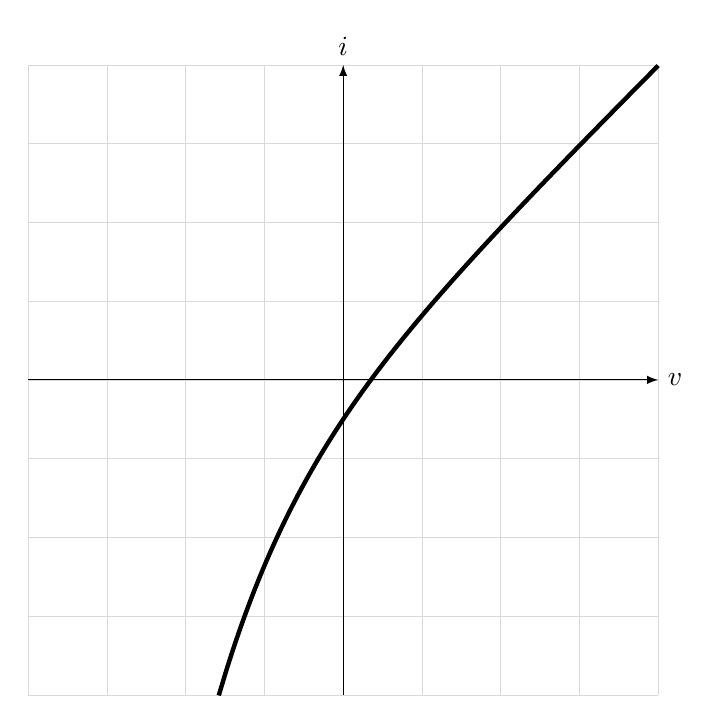
\begin{tikzpicture}
			\draw[help lines, color=gray!30] (-4,-4) grid (4,4);
			\draw[-latex] (-4,0)--(4,0) node[right]{$v$};
			\draw[-latex] (0,-4)--(0,4) node[above]{$i$};
			\draw[ultra thick,black] plot[domain=-1.58:4, samples = 50, smooth]({\x}, {-(1/2)*exp(-\x)+\x});
		\end{tikzpicture}
		\caption{De \((v,i)\)-karakteristiek van de niet-lineaire component.}
		\label{fig:nietlineair}
	\end{figure}

\end{document}


























